\documentclass[11pt,twoside,a4paper]{article}
\usepackage{graphicx}
\begin{document}
\title{RDC}
\author{Roberto Alcover Couso}
\date{20/9/2018}
\maketitle

\section*{Introduction}
In this document we will explain how to implement RDC in python and the reasons behind the implementation decisions aswell as some hints of the theory behind it which is necessary to understand in order to implement this method.
\section*{Theory behind it}
\subsection*{Estimation of Marginal Observation Ranks}
\textbf{Using uniform variables}

Consider a random vector X = (X\small{1} , . . . , X\small{d} ) with continuous marginal cumulative distri-
bution functions (cdfs) P\small{i}, 1$\leq$i$\leq$d. 
\textbf{U}=(U\small{1},...,U\small{d}):=(P\small{1}(X\small{1}),...,P\small{d}(X\small{d})) has uniform marginals.(\textit{Probability Integral Transform [Appendix 1.1]})

\begin{flushleft}
\textbf{Using the ecdfs}

Let X\small{1},...,X\small{n} be iid random variables qith common cumulative distribution function P. Then, the empirical cumulative distribution function, defined as
\end{flushleft}
\centering{
$$P_{n} := \frac{1}{n} \sum_{i=1}^{n} \textit{I}(X_{i} \leq x)$$
}
\begin{flushleft}
converges uniformly to P:
\end{flushleft}
$$\|P_{n} - P\|_{\infty}= \sup_{x \in R}|P_{n}(x) - P(x)| \rightarrow^{a.s} 0 $$
(\textit{Appendix 1.2})

\begin{flushleft}
\textbf{Generation of Random Non-Linear Proyections}

Thanks to Rahimi-Brecht axiom one can achive regressors of the form $\sum_{i=1}^{K} \alpha_{i}\phi(wi)$ when we randomize over the weights wi inside the non-linearities $\phi$ but optimize the lineat mixing coefficients $\alpha$.
Let $w_{i}\sim \mathcal{N}(\textbf{0}, s\textbf{I}), b_{i}\sim\mathcal{U}[-\pi,\pi].$
Given a data collection \textbf{X} = (x\small{1},...,x\small{n}), we will denote by
\end{flushleft}
$\Phi(\textbf{X};k,s):=
\left(\begin{array}{ccc} \phi(w_{1}^{T}x_{1} + b_{1})	&	...	&	\phi(w_{k}^{T}x_{1} + b_{k}) \\
. & . & . \\
. & . & . \\
. & . & .\\
\phi(w_{1}^{T}x_{n} + b_{1}) & ... & \phi(w_{k}^{T}x_{n} + b_{k}) \end{array}\right)$



\begin{flushleft}

\textbf{Canonical Correlation Analysis}

We will use CCA to compute the linear combinations of the augmented empirical copula that have maximal correlation.
CCA searches for vectors a and b which maximize the correlation $\rho_{a^TXb^TY}$

(\textit{Appendix 1.3})
\section*{Appendixes}
\subsection*{Appendix 1.1 Probability Integral Transform}
Let X with CDF F and Y = F(X), then Y follows a uniform distribution.
$F_{Y}(y)=P(Y\leqy)=P(F_{X}(x)\leq y) = P(X\leqF^{-1}_{X}(y)) = F_{X}(F^{-1}_{X}(y)) = y$
\subsection*{Appendix 1.2 Glivenko-Cantelli Theorem}
$$F_{n} := \frac{1}{n} \sum_{i=1}^{n} \textit{I}(X_{i} \leq x)$$ converges uniformly to P:
Let X = ($x_{0},...,x_{m}$) such that $-\infty = x_{0}<x_{1}< ... <x_{m}=\infty$ and $ F(x_{j}) - F(x_{j-1}) \leq \frac{1}{m}$
$F_{n}(x)-F(x)\leq F_{n}(x_{j})-F(x_{j-1}) = F_{n}(x_{j})-F(x_{j}) + \frac{1}{m}$
$F_{n}(x) - F(x) \geq F_{n}(x_{j-1}) -F(x_{j}) = F_{n}(x_{j-1}) -F(x_{j-1}) - \frac{1}{m}$
\end{flushleft}
$$\|F_{n} - F\|_{\infty}= \sup_{x \in R}|F_{n}(x) - F(x)| \leq \max_{j \in {1,..,m}}|F_{n}(x_{j})-F(x_{j})| + \frac{1}{m} \rightarrow 0 (a.s)$$
\begin{flushleft}
\subsection*{Appendix 1.3 CCA}

Let us consider the correlation $\phi(a,b)$ between the two prohections in more detail. Suppose that:

\left(\begin{array}{cc} X \\ Y \end{array}\right) $\sim$
\left(\begin{array}{cc} \left(\begin{array}{cc} $\mu$ \\ $\nu$\end{array}\right) & \left(\begin{array}{cc} $\Sigma_{XX}$ & $\Sigma_{XY}$ \\
$\Sigma_{YX}$ & $\Sigma_{YY}$\end{array}\right)\end{array}\right)

Then:

$\phi(a,b) = \frac{a^{T}\Sigma_{XY}b}{(a^{T}\Sigma_{XX}a)^{1/2}(b^{T}\Sigma_{YY}b)^{1/2}}$

Which is easy to see that:
$\phi(a,b) = \phi(ca,b)$ for any c.
Therefore the problem of maximizing $\phi$ can be realiced under the constrains:

$a^{T}\Sigma_{XX}a = 1$
$b^{T}\Sigma_{YY}b = 1$.

First we need to define:
$\mathbb{K} = \Sigma_{XX}^{-1/2}\Sigma_{XY}\Sigma_{YY}^{-1/2}$
which its eigenvalues will be the canonical correlation coefficients.

\textit{k = rank($\mathbb{K}) = rank(\Sigma_{XY}}$), we will use this in the implementation}

\subsection*{Appendix 1.4 Python Code}
In order to create the data which we will be applying RDC we will base on the numpy library.
X $\sim \mathcal{U}[0,1]$ which will be implemented thoughout the function np.random.rand(). In order to generate different samples each execution we will provide a seed which is going to change every time the program is executed(for example current time).
Y will be generated by applying different functions to the random vector X.
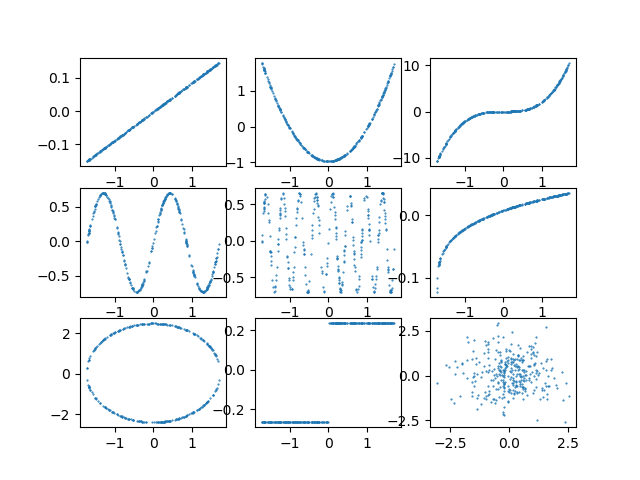
\includegraphics{Figure_1}

The code for the rdc itself its pretty simple:

\textit{First we will apply the ecdf function to the vectors (which is needed to be implemented separately in python) and concatenate the column full of ones in order to generate the bi later on.}	

	lx = len(x)

	ly = len(y)

	x = np.concatenate((ecdf(x).reshape(-1,1),

		np.ones(lx).reshape(-1,1)),axis=1)

	y = np.concatenate((ecdf(y).reshape(-1,1),

		np.ones(ly).reshape(-1,1)),axis=1)	

	nx = x.shape[1]

	ny = y.shape[1]
	
\textit{Then we generate a matrix with the samples of the w $\sim \mathcal{N}(0,1)$ in order to multiply it and generate the desired matrix explaned in the section Generation of Random Non-Linear Proyections}

	wx = norm(nx*k,s).reshape(nx,k)
	
	wy = norm(ny*k,s).reshape(ny,k)

	wxs = np.matmul(x,wx)
	
	wys = np.matmul(y,wy)
	
\textit{we apply the function $\phi$ which is in this case is a sin}

	fX = np.sin(wxs)

	fY = np.sin(wys)
	
\textit{cancor function will be explained later on in this brief}

	res = cancor(fX,fY,k)
	
\textbf{Cancor function}

As we see in the paper by David Lopez-Paz, Philip Hennig and Bernhard Schölkopf the correlation coefficient will be tightly related to the f,k and s parameters.
While implementing this some problems related to numerical problems while calculating the inverse of Cxx and Cyy showed up. If the value of k is too big then the rank of fX or fY could be smaller than k, therefore we need to find the largest k which makes the eigenvalues real-valued.
We will implement this through a binary search of k, although is not the most efficient way of solving this problem is the simplest way.


\textit{First we will calculate the covariance matrix}
	
	C = np.cov(np.hstack([x, y]).T)

\textit{Now we will apply the binary search for the optimum k value in which the Cxx and Cyy are not singular}
	
	k0 = k
	lb = 1
	ub = k

\textit{Due to calculations of the optimum k sometimes becomes a double, therefore not being able to index a matrix}

	while True:
	
	
\hspace*{50}		k = int(k)
		
\textit{We will calculate the new cancor using the new values of k leaving behind some variations which due to numerical aproximation of functions by the computers may create some rows equal}

\hspace*{50}		Cxx = C[:k,:k]

\hspace*{50}		Cyy = C[k0:k0+k, k0:k0+k]

\hspace*{50}		Cxy = C[:k, k0:k0+k]

\hspace*{50}		Cyx = C[k0:k0+k, :k]

\hspace*{50}		eigs = np.linalg.eigvals(np.dot(np.dot(np.linalg.inv(Cxx), Cxy),

	\hspace*{50}	                                np.dot(np.linalg.inv(Cyy), Cyx)))

\textit{If k is too big, the values of the eigenvalues won't be real between 0 and 1}

\hspace*{50}		if not (np.all(np.isreal(eigs)) and

\hspace*{50}\hspace*{25}				0 <= np.min(eigs) and

\hspace*{50}\hspace*{25}				np.max(eigs) <= 1):

\hspace*{50}\hspace*{50}			ub -= 1

\hspace*{50}\hspace*{50}			k = (ub + lb) / 2

\hspace*{50}\hspace*{50}			continue

\hspace*{50}		if lb == ub: break

\hspace*{50}		lb = k

\hspace*{50}		if ub == lb + 1:

\hspace*{50}\hspace*{50}			k = ub

\hspace*{50}		else:

\hspace*{50}\hspace*{50}			k = (ub + lb) / 2

	return np.sqrt(np.max(eigs))
	
\end{flushleft}
\left(\begin{array}{cc} 1 & 0.5 \\ 0.5 & 1\end{array} )
\end{document}
